\documentclass[12pt]{extarticle}
\usepackage[utf8]{inputenc}
\usepackage[english,russian]{babel}
\usepackage{vmargin}
\usepackage{indentfirst}
\usepackage[T2A]{fontenc}
\usepackage{graphics}
\usepackage{amsthm}
\usepackage{amsbsy}
\usepackage{amsmath}
\usepackage{amssymb}
\usepackage{amsfonts}
\usepackage{mathtext}
\usepackage[pdftex,a4paper,colorlinks,linkcolor=blue,citecolor=blue]{hyperref}	

\usepackage{mathtext}
\usepackage{mathenv}
\usepackage[pdftex]{graphicx}
\usepackage{array}
\usepackage{graphicx,xcolor}
\usepackage{xcolor}
\usepackage{float}
\usepackage{longtable}

%\parindent = 30pt
%\hoffset = 0pt
%\voffset = 0pt
\oddsidemargin = 100pt
\topmargin = 18pt
%\headheight = 12pt
%\headsep = 25pt
\textheight = 700pt
\textwidth = 440pt
%\marginparsep = 10pt
%\marginparwidth = 103pt

\usepackage{tikz}
\usepackage{verbatim}

\paperwidth = 597pt
\paperheight = 845pt
\numberwithin{equation}{section}

\DeclareMathOperator{\sign}{sign}
\DeclareMathOperator{\const}{const}
\renewcommand{\Re}{\mathop{\mathrm{Re}}\nolimits}
\renewcommand{\Im}{\mathop{\mathrm{Im}}\nolimits}
\newtheorem{algorithm}{Алгоритм}[section]

\begin{document}

\begin{titlepage} \newpage 
\begin{center} МОСКОВСКИЙ ГОСУДАРСТВЕННЫЙ УНИВЕРСИТЕТ ИМ. М.В. ЛОМОНОСОВА\end{center} 
\vspace{8em} \begin{center} 
\Large Механико-математический факультет \\ \end{center}
\vspace{2em} \begin{center} 
\textsc{Отчет по практикуму на ЭВМ \linebreak 
\textbf{еботня какая-то}} \end{center}
\vspace{6em} \newbox{\lbox} \savebox{\lbox}{\hbox{Д.Салахов}} 
\newlength{\maxl} \setlength{\maxl}{\wd\lbox} \hfill\parbox{12	cm}
{ \hspace*{10cm}\hspace*{-5cm}Студент 4 курса:\hfill\hbox to\maxl{Дамир}\\
\hspace*{10cm}\hspace*{-5cm}Преподаватель:\hfill\hbox to\maxl{Ченцова}}\\  \vspace{\fill}
\begin{center} Москва \\ 2017\end{center} \end{titlepage}

%\maketitle

%\renewcommand{\contentsname}{Содержание}
\tableofcontents
\renewcommand{\figurename}{График}
\renewcommand{\theequation}{\thesection.\arabic{equation}}


\newpage

\section{Постановка задачи} \label{sec:1-postanovka-zadachi}
Дано уравнение в частных производных с заданными начальными условиями:
\begin{equation}
\left\{
	\begin{aligned}
&\frac{\partial u}{\partial t} = \frac{\partial ^2 u}{\partial t^2} + u^3 - \cos \frac{\pi x}{2} \\
& x = 0: \qquad \frac{\partial u}{\partial x} = 0\\
& x = 1: \qquad u = 0 \\
	\end{aligned}
\right.
\label{eq:1-nachal-zadacha}
\end{equation}

Неизвестная функция -- $u$ от двух переменных $t$ и $x$ (переменные Эйлера), причем $$(t, x) \in Q = [0, 1] \times [0, 1].$$

Само уравнение можно перепиать в виде
\begin{equation}
\frac{\partial u}{\partial t} = \frac{\partial ^2 u}{\partial t^2} + f, \label{eq1}
\end{equation}
где $f$ -- данная функция.

Для начального момента  времени задана функция $u_0$, значения которой совпадают со значениями $u$ на отрезке $x \in [0; 1]$:
\begin{equation}
u |_{t=0} = u_0 = 0.9 \cdot (1 - x^2), \label{nu}
\end{equation}

Для решения задачи введем равномерную сетку $\omega_h$ с шагом $h$ по оси $x$ и с шагом $\tau$ по оси $t$. 
Введем константы $M$ и $N$, такие что $X = Mh$ и $T = N\tau$.

\section{Описание схемы} \label{scheme}
Для поиска численного решения задачи \ref{eq:1-nachal-zadacha} будем использовать разностную схему, в которой при аппроксимации членов используются односторонние разности:
%\begin{aligned}
%\left\{
	\begin{align}
		&V_t= V_{x \hat x} + f,\qquad x \in \omega_h, \label{eq1-1}\\
		&V_{x, 0} = 0 \label{eq1-2}\\
		&{V^n_M} = 0 \label{eq1-3}
	\end{align}
%\right.
%\end{aligned}
Исходя из \ref{nu}, в качестве значений решения на нулевом слое берутся проекции на сетку $\bar{\omega}_h$ функции $u_0$, т.е.
$$V_m^0 = (u_0)_m, \qquad \mbox{где} \quad m = 0, 1, \dots M.$$

Коэффициенты перед элементами $V$ в уравнении \ref{eq1-1} задают элементы матрицы и правой части.
Таким образом с помощью этих уравнений можно получить матричное, решив которое, можно найти значения для функции $u$ на новом слое сетки.
Распишем уравнения системы для нахождения элементов матрицы.

\subsection{Уравнение \ref{eq1-1}}
Вспомним обозначения:
\begin{align}
&V_t = \cfrac{V_m^{n+1} - V_m^n}{\tau} \label{eq2:1:1}\\
&V_{x \hat x} = \cfrac{V_{m+1}^{n+1} - 2V_m^{n+1} + V_{m-1}^{n+1}}{h^2} \label{eq:2:1:2}
\end{align}

Перепишем само уравнение:
$$\cfrac{V_m^{n+1} - V_m^n}{\tau} = \cfrac{V_{m+1}^{n+1} - 2V_m^{n+1} + V_{m-1}^{n+1}}{h^2} + f
$$
Приводя подобные и домножая обе части на $\tau$ и взяв $\gamma = \tau/h$
\begin{equation}
 V_{m+1}^{n+1} \cdot \cfrac{\gamma}{h} + V_m^{n+1} \cdot \left( -1 - \cfrac{2\gamma}{h}\right) + V_{m-1}^{n+1} \cdot \cfrac{\gamma}{h} = -V_m^n - f \cdot \tau
 \label{eq2:1:final}
\end{equation}

\subsection{Уравнение \ref{eq1-2}}
Из уравнения \ref{eq1-2} получаем коэффициенты для нулевой строки матрицы и правой части алгебраической задачи.
\begin{align*}
&V_{x, 0} = \cfrac{V_1^{n+1} - H_0^{n+1}}{h}\\
\end{align*}
Итого, домножив на $h$ получим
\begin{equation}
-V_0^{n+1} + V_{1}^{n+1} = 0 \label{eq:2final}
\end{equation}

\subsection{Уравнение \ref{eq1-3}}
Из этого уравнения получаем последню строку матрицы (она нулевая).

\subsection{Алгоритм}
На каждом шаге итерации сначала будем строить матрицу размера $M+1$ и правую часть для нового слоя $V^{n+1}$, используя уравнения \ref{eq2:1:final}, \ref{eq:2final}, \ref{eq1-3}.
Решив полученную систему линейное уравнение, найдем новое приближение для $u$.

Заметим, из итоговых уравнений видно, что в алгебраической задаче получились трехдиагональные матрицы.
Таким образом, полученную СЛУ можно решить методом прогонки.

\newpage
\appendix \label{grap1}
\section{Для $f=u^3$} 
\begin{figure}[H]
\begin{minipage}[h]{0.43\linewidth}
\center{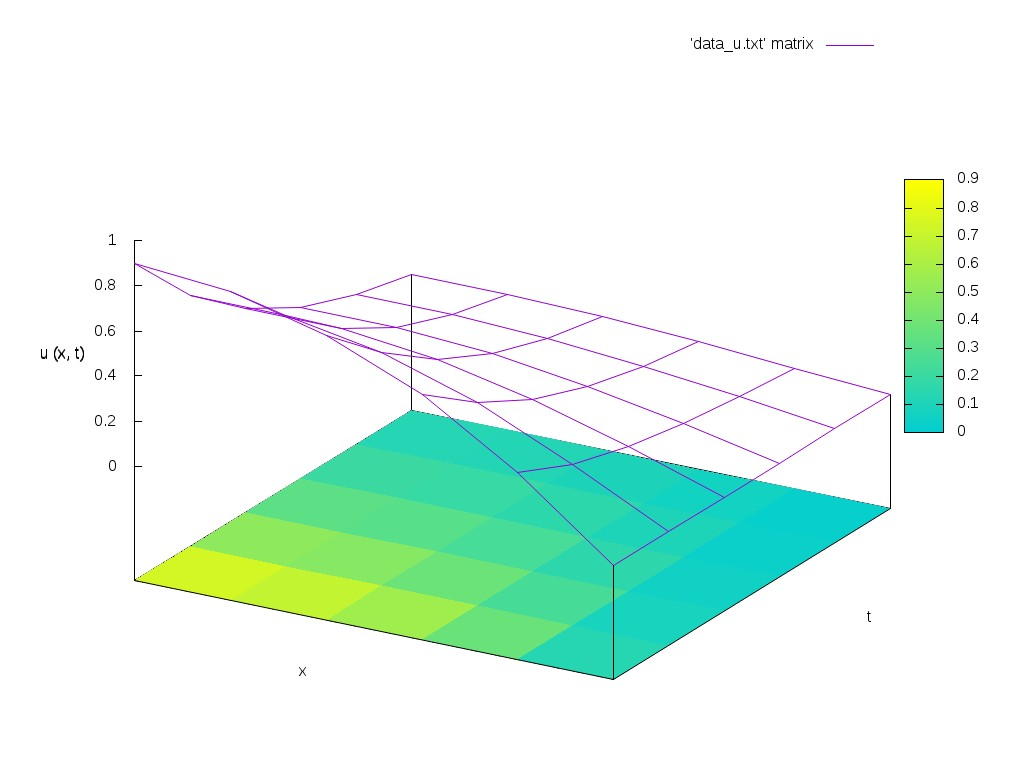
\includegraphics[width=1\linewidth]{../u/lines5x5.jpg}} $N=5; M=5$ \\
\end{minipage}
\hfill
\begin{minipage}[h]{0.43\linewidth}
\center{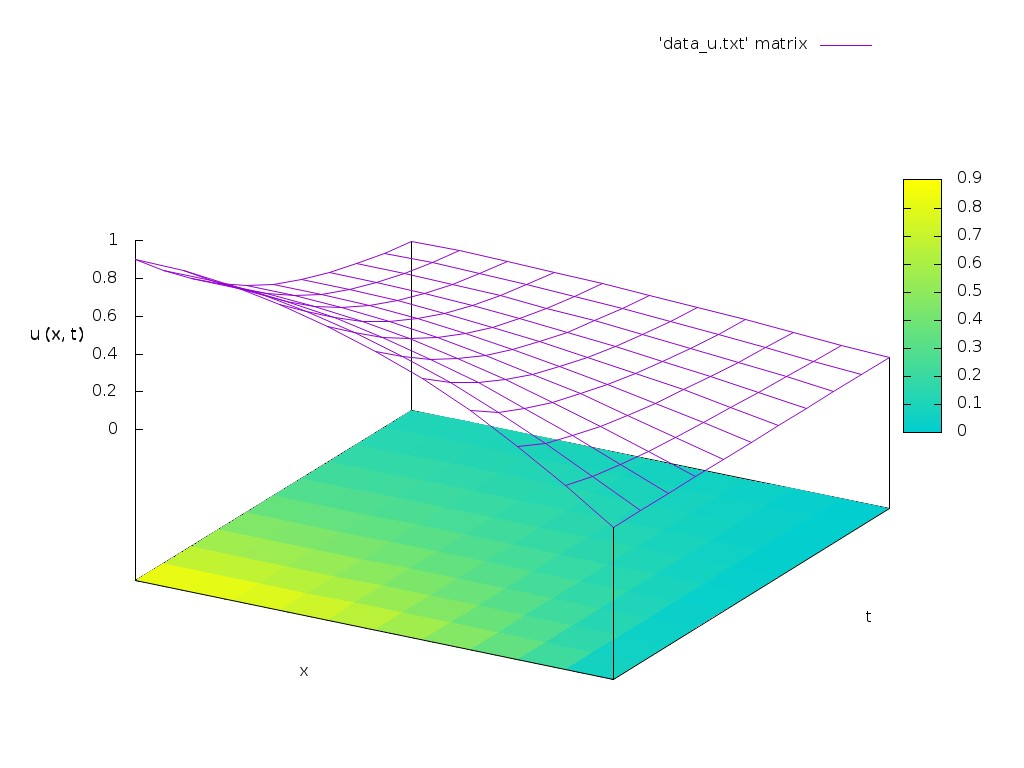
\includegraphics[width=1\linewidth]{../u/lines10x10.jpg}} $N=10; M=10$ \\
\end{minipage}
\end{figure}

\begin{figure}[H]
\begin{minipage}[h]{0.43\linewidth}
\center{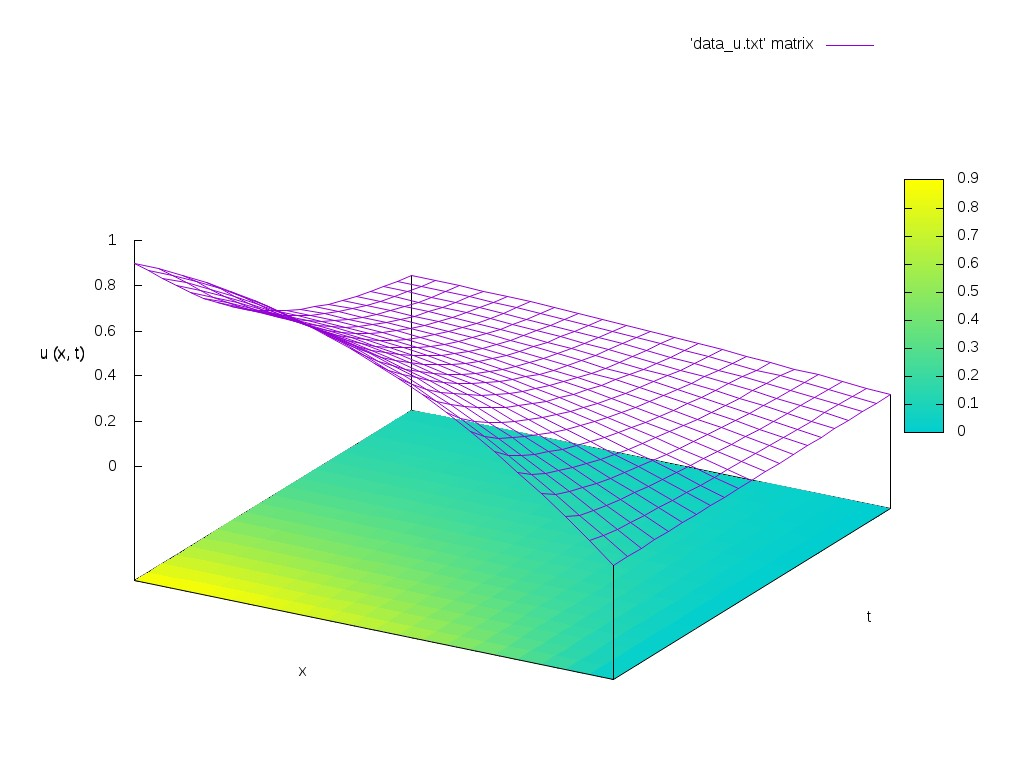
\includegraphics[width=1\linewidth]{../u/lines20x20.jpg}} $N=20; M=20$ \\
\end{minipage}
\hfill
\begin{minipage}[h]{0.43\linewidth}
\center{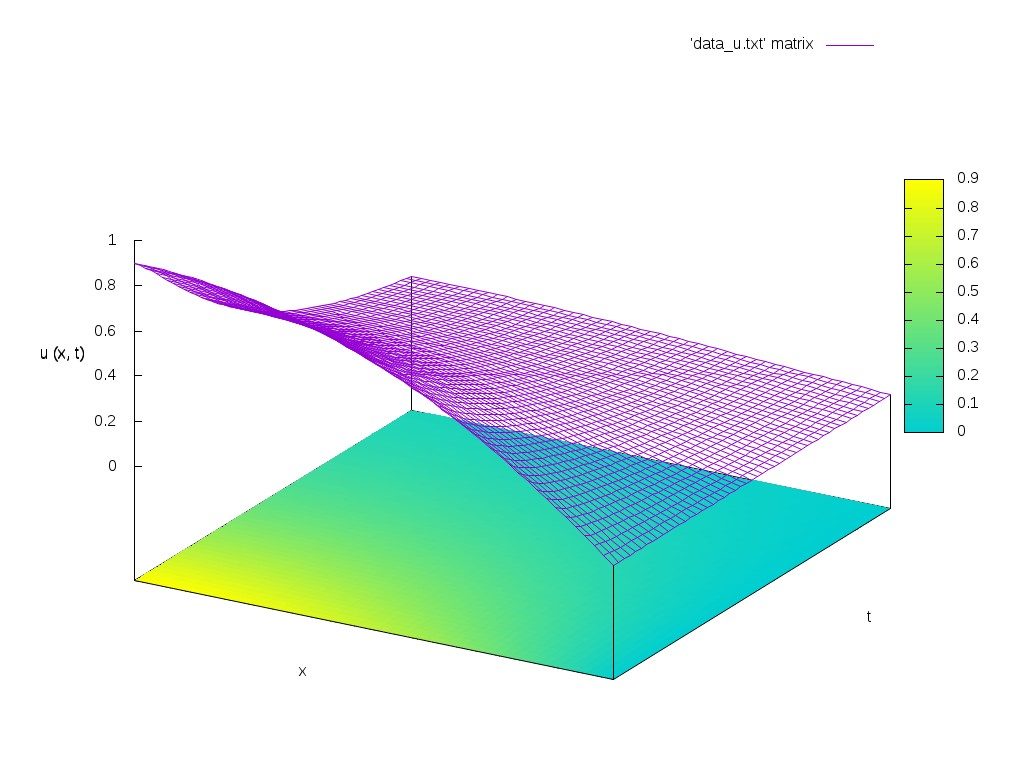
\includegraphics[width=1\linewidth]{../u/lines50x50.jpg}} $N=50; M=50$ \\
\end{minipage}
\end{figure}

\begin{figure}[H]
\begin{minipage}[h]{0.43\linewidth}
\center{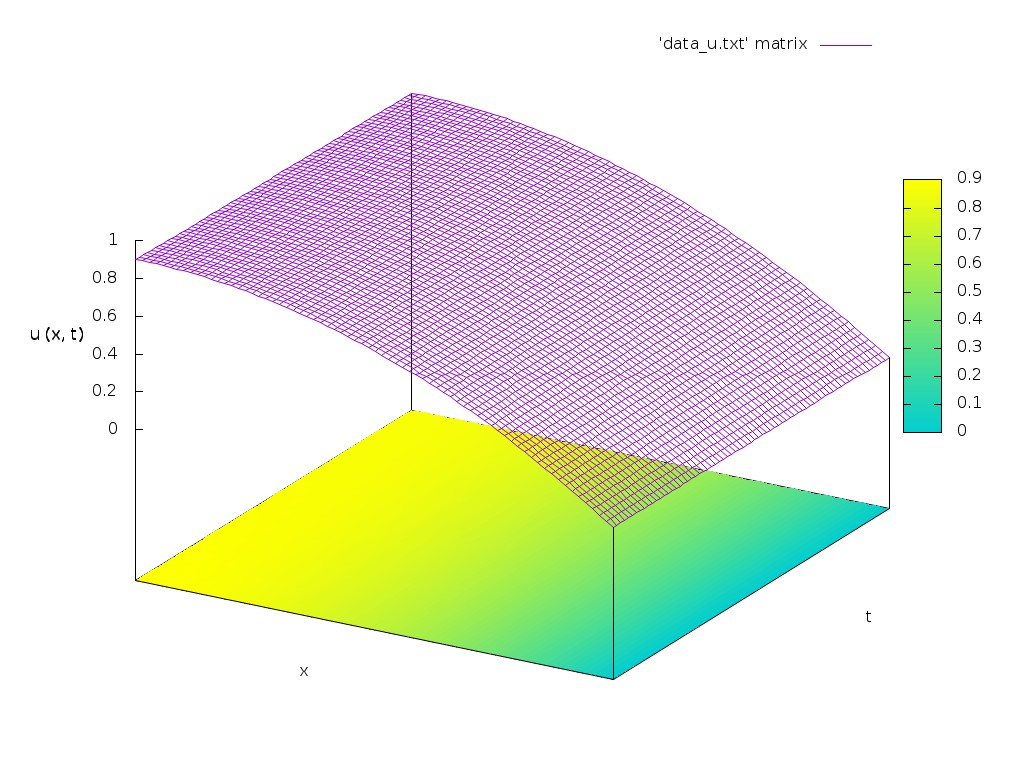
\includegraphics[width=1\linewidth]{../u/lines70x70.jpg}} $N=70; M=70$ \\
\end{minipage}
\hfill
\begin{minipage}[h]{0.43\linewidth}
\center{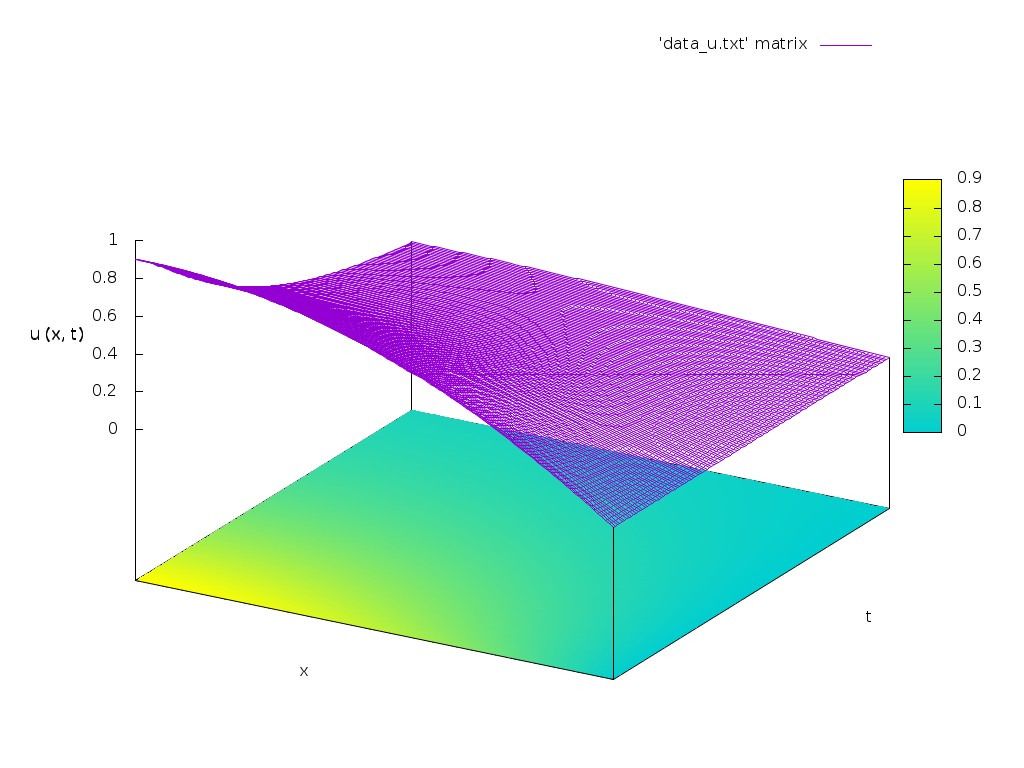
\includegraphics[width=1\linewidth]{../u/lines120x120.jpg}} $N=100; M=100$ \\
\end{minipage}
\end{figure}


\section{Для $f=u^3 - \cos \frac{\pi x}{2}$} 
\begin{figure}[H]
\begin{minipage}[h]{0.43\linewidth}
\center{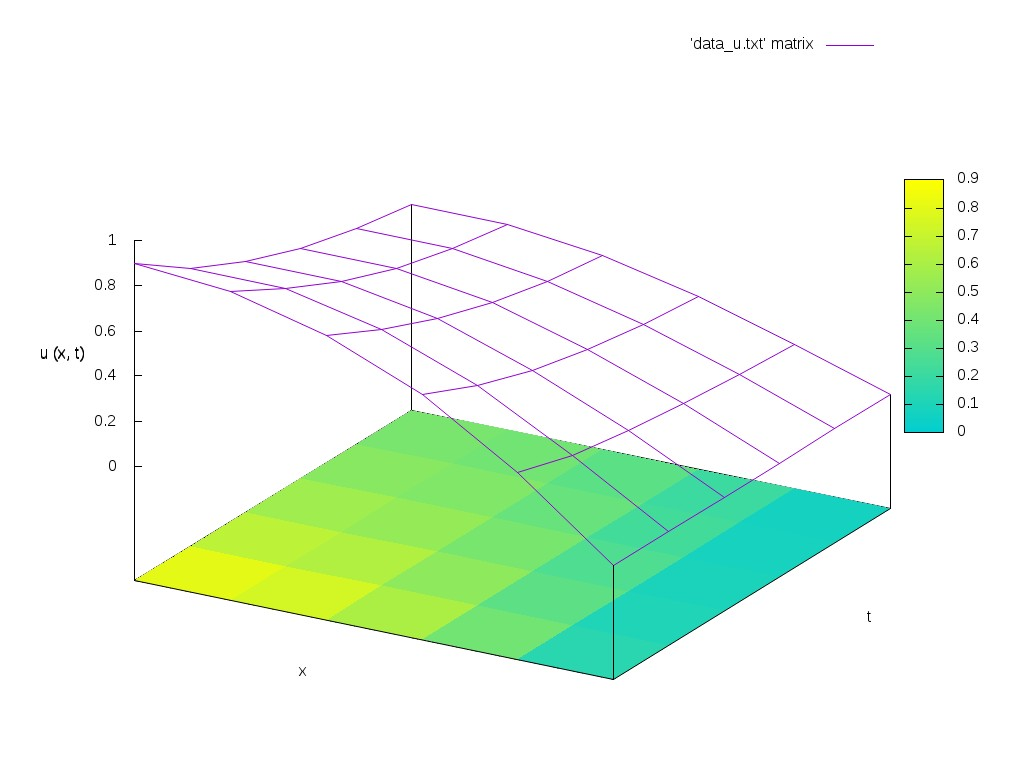
\includegraphics[width=1\linewidth]{../u-cos/lines5x5.jpg}} $N=5; M=5$ \\
\end{minipage}
\hfill
\begin{minipage}[h]{0.43\linewidth}
\center{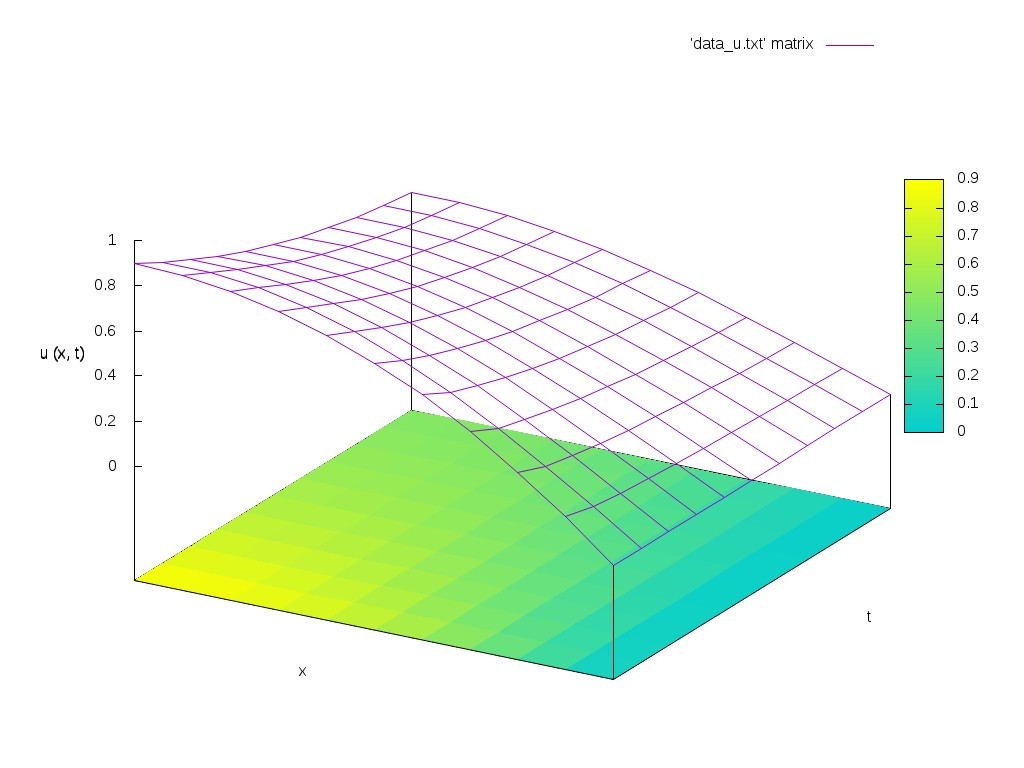
\includegraphics[width=1\linewidth]{../u-cos/lines10x10.jpg}} $N=10; M=10$ \\
\end{minipage}
\end{figure}

\begin{figure}[H]
\begin{minipage}[h]{0.43\linewidth}
\center{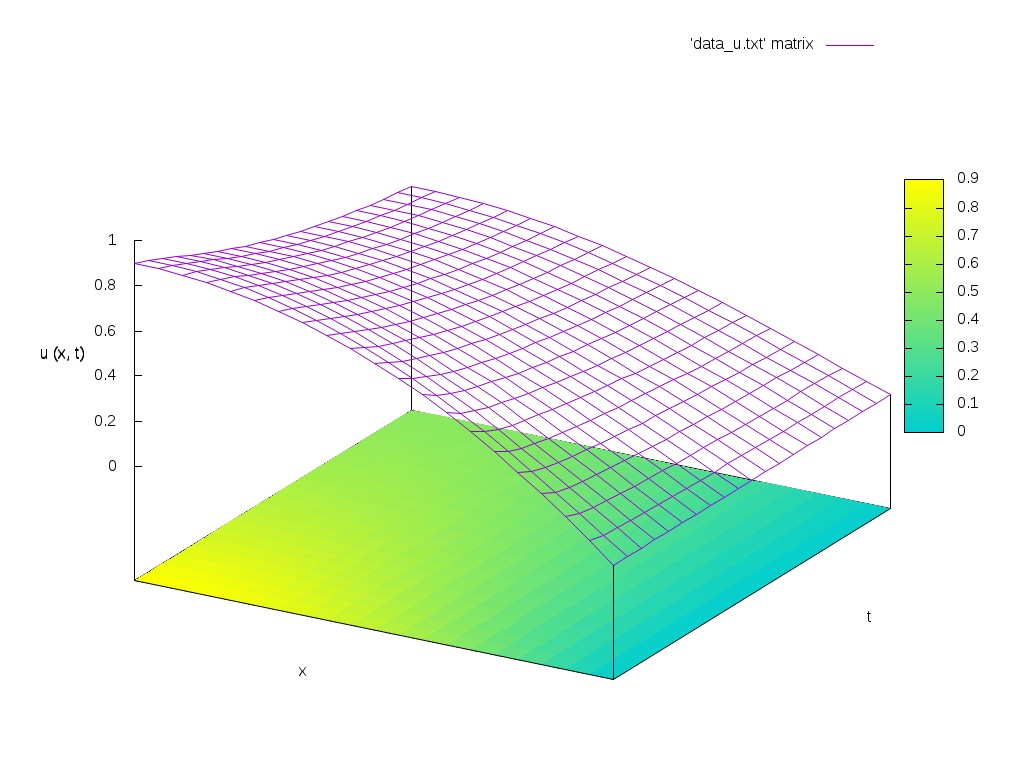
\includegraphics[width=1\linewidth]{../u-cos/lines20x20.jpg}} $N=20; M=20$ \\
\end{minipage}
\hfill
\begin{minipage}[h]{0.43\linewidth}
\center{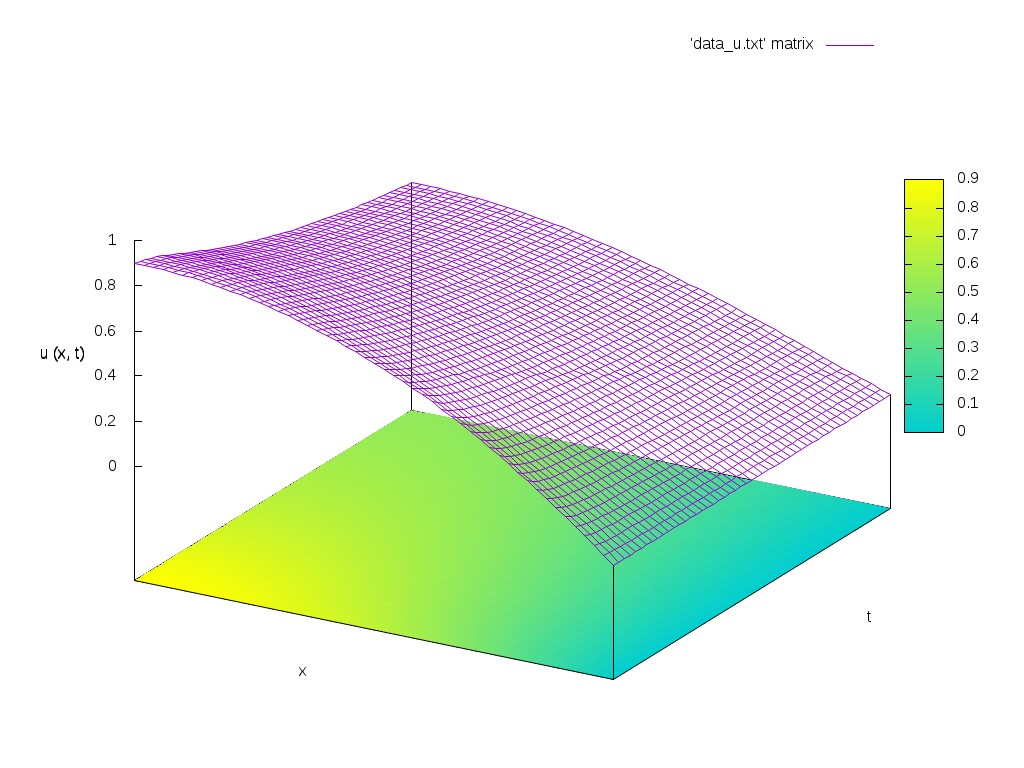
\includegraphics[width=1\linewidth]{../u-cos/lines50x50.jpg}} $N=50; M=50$ \\
\end{minipage}
\end{figure}

\begin{figure}[H]
\begin{minipage}[h]{0.43\linewidth}
\center{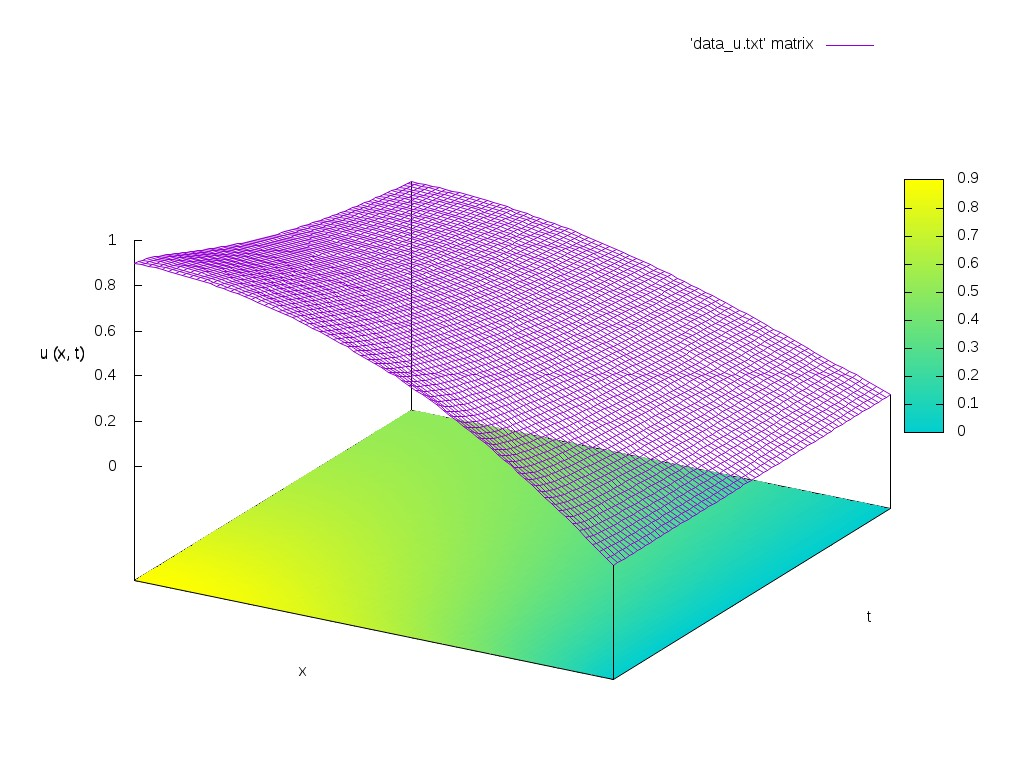
\includegraphics[width=1\linewidth]{../u-cos/lines70x70.jpg}} $N=70; M=70$ \\
\end{minipage}
\hfill
\begin{minipage}[h]{0.43\linewidth}
\center{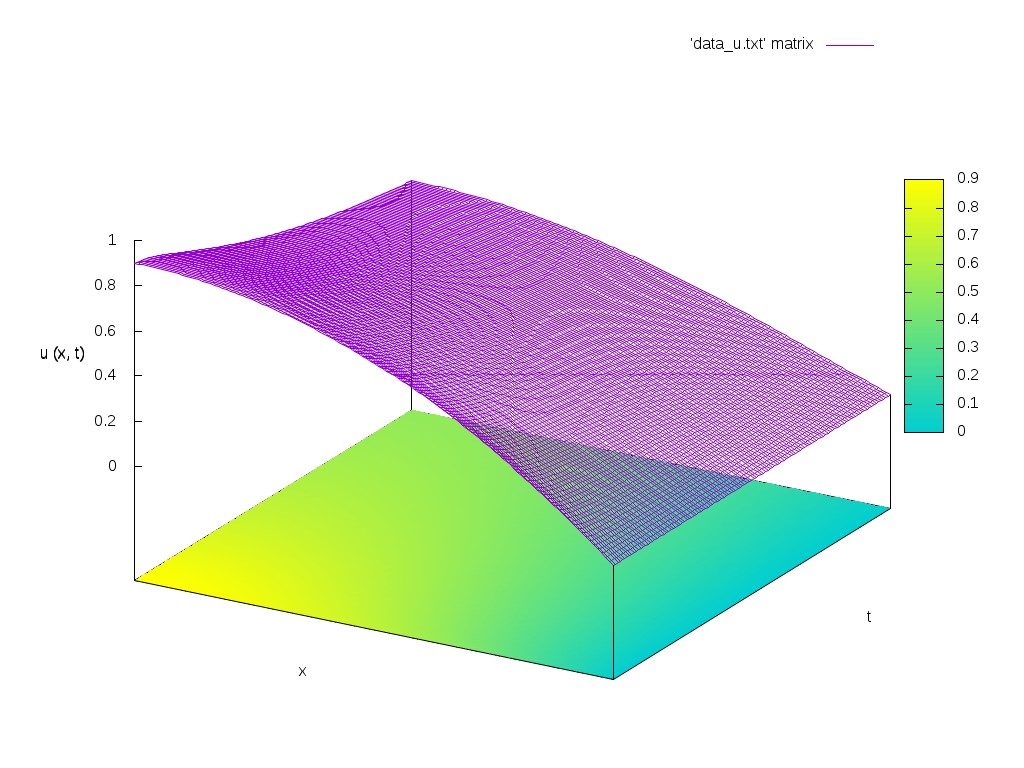
\includegraphics[width=1\linewidth]{../u-cos/lines120x120.jpg}} $N=100; M=100$ \\
\end{minipage}
\end{figure}

\end{document}